%% V1.0
%% by Christopher Leith, udacl@cielsystems.com
%% This is a template for Udacity projects using IEEEtran.cls

\documentclass[10pt,journal,compsoc]{IEEEtran}

\usepackage[pdftex]{graphicx}    
\usepackage{cite}
\hyphenation{op-tical net-works semi-conduc-tor}

\begin{document}

\title{MapMyWorld - Robotic Simultaneous Localization and Mapping}

\author{Christopher Leith}

\markboth{MapMyWorld, SLAM, Udacity}%
{}
\IEEEtitleabstractindextext{%

\begin{abstract}
In this project we create a simulated robot and demonstrate Simultaneous Localization and Mapping (SLAM) within the ROS framework to permit navigation within a small simulated "Gazebo" world. A differential drive robot is designed to operate within the Gazebo simulation and uses the ROS navigation stack and the RTAB-map-ros package for creating a map on the fly and localizing itself within that map.\end{abstract}

% Note that keywords are not normally used for peerreview papers.
\begin{IEEEkeywords}
Mobile Robot, SLAM, ROS.
\end{IEEEkeywords}}


\maketitle
\IEEEdisplaynontitleabstractindextext
\IEEEpeerreviewmaketitle
\label{sec:Introduction}
\section{Introduction}
\IEEEPARstart{M}{obile} robots must be able to determine their location within their region of operation, a process known as localization, and navigate to other locations reliably in order to perform their tasks successfully.

If there is no predefined map of the region the robot must be able to build up a map of using its' sensors and simultaneously localize itself within that map. This process is known as Simultaneous Localization and Mapping (SLAM).

In this project SLAM is demonstrated in a ROS/Gazebo simulation environment with both supplied Gazebo world and a custom designed world. For each world the robot is spawned in the simulated space and driven by the keyboard 'teleop' control around that world. The robot sensors' data streams are supplied to the RTABMap module that performs the SLAM process on that data and slowly builds both 2D and 3D maps of the world and computes the robots pose within that world. These maps can be visualized in RViz and RTABMapViz.

\section{Background / Formulation}
Because mapping and localization is so important for mobile robotics it is a highly researched field and has many well developed techniques and technologies. The SLAM approach has proven a very effective solution for this problem and has evolved into a family of similar techniques including Fast-SLAM, Graph-Slam and occupancy grid mapping, each with with pros and cons for different applications. 

Occupancy grid mapping is a technique that uses bayes filtering to determine the presence of obstacles within a 2D grid of the environment.

FastSlam uses particle filtering. It uses comparisons of kalman filtered random particle poses against only the the current, known sensor data input at each moment.

GraphSlam solves the Slam problem by analyzing the entire trajectory of robot poses, all of the previous sensor inputs and the current map. It attempts to correlate the sensor inputs into correlated features that then feedback into correcting the  presumably noisy pose locations. This is the technique used by by RTABMap.

\subsection{RTABMap Slam}
In this project we demonstrate a mature SLAM framework implementation known as Real-Time Appearance-Based Mapping (RTAB-Map) available for 'plug-and-play' use in the ROS robotic framework. RTABMap is a graph-based SLAM implementation intended for robots operating for long periods in large environments. Internally it uses many techniques to efficiently accumulate large maps in real time even on the constrained computing resources typically available on mobile robotic hardware. In this project the RTABMap uses 3 sensor streams:

\begin{itemize}
 \item Wheel Odometry
 Measures the distance traveled be each wheel.
 \item Hokuyo Laser Rangefinder
 Mounted on top of the cylinder.
 \item RGB-Depth Camera
 Mounted on the front of the cylinder.
\end{itemize}

The RTABMap package uses all of these sensor data streams in a way that is, frankly, somewhat opaque. It is primarily the RGB-D point cloud data that is used by the RTABMap package to detect visual features over the course of mapping whose geometric similarities correspond closely enough to infer that they must be images of the same feature. The detection of such a correspondence is called a 'loop closure'. As loop closures are determined they can be used reconcile the locations of seemingly disparate stored image features, as determined by odometry, into identical features of the map and thereby correct path inaccuracies due to noise of the odometry. Whether a loop closure is determined or not the new images are stored for later camparisons. As the dictionary of stored image features grows the processing load increases. RTABMap implements several data caching strategies to ensure that real time processing can continue.


\section{Configuration}
Much of the configuration of this ROS project was carried over from the prior Localization project and was adapted as described below.The ROS graph is shown in Fig ~\ref{fig:rosgraph}.

\begin{figure}[h]
      \centering
      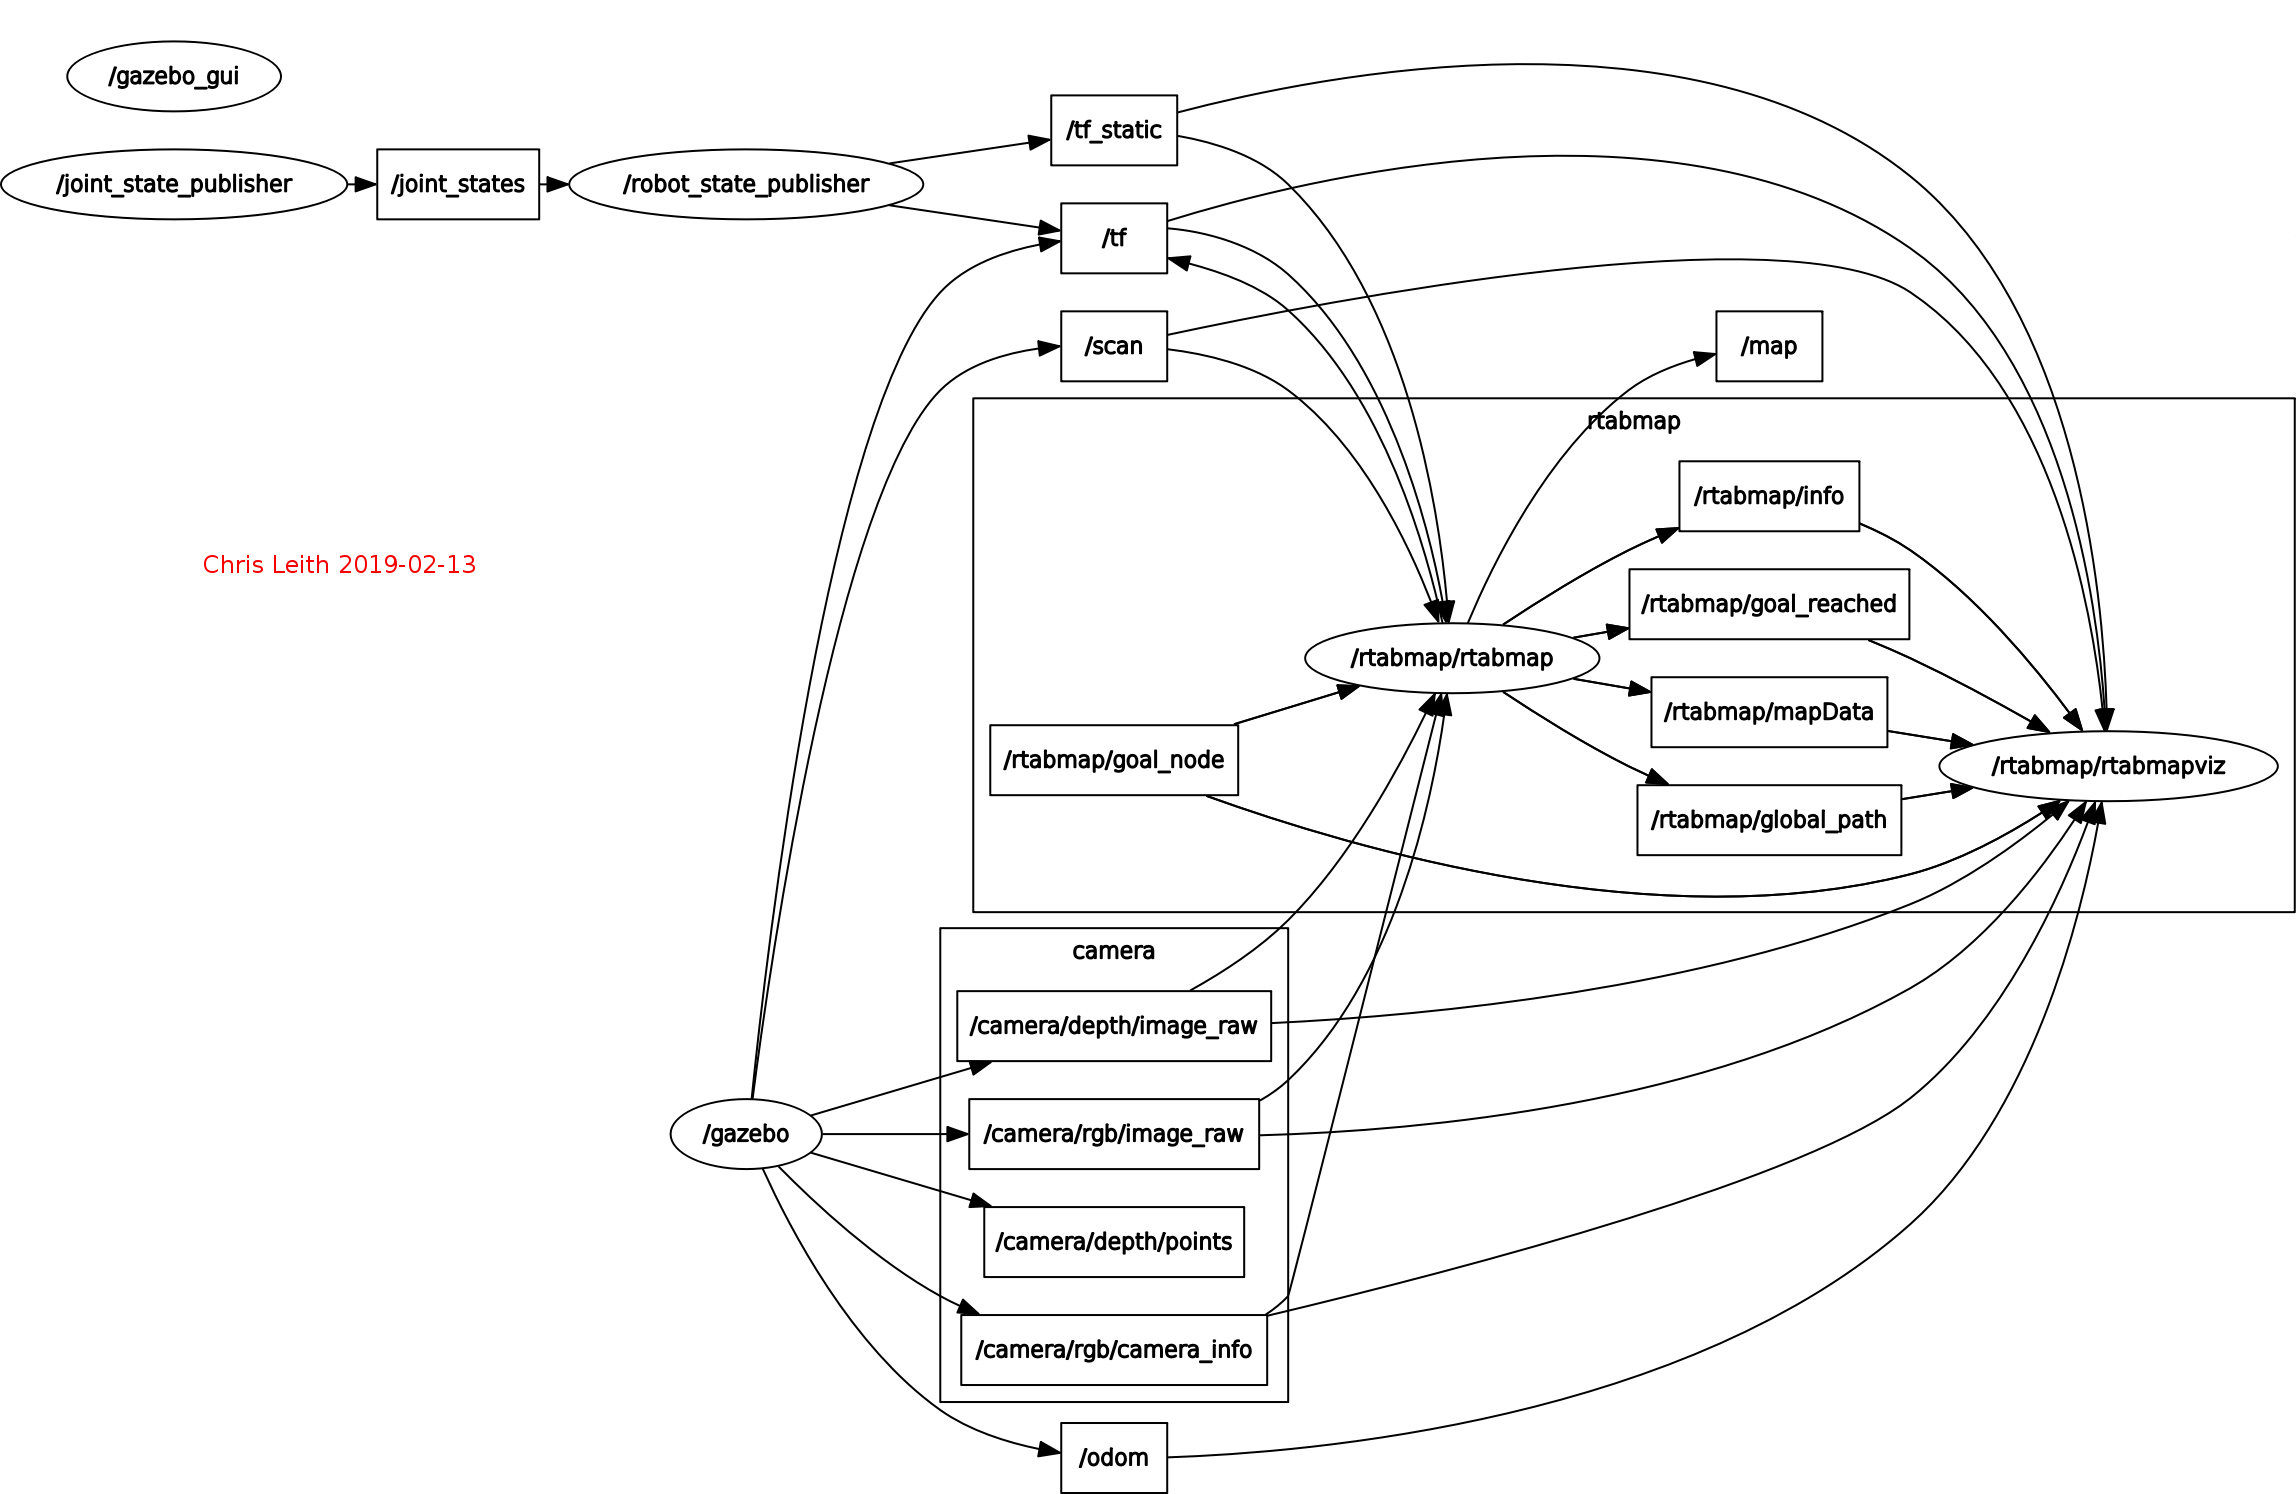
\includegraphics[width=\linewidth]{Assets/rosgraph_working.png}
      \caption{CielBot nodes and topics ROS Graph}
      \label{fig:rosgraph}
\end{figure}

\subsection{RTABMap Config}
 The configuration for the RTABMap ROS package was supplied and only minor modifications were required to link up the data stream ROS topics correctly. Unfortunately all available time was taken up achieving basic functionality and the default values had to remain as is. However it clear that many parameters of RTABMap should be tuned to optimized the effectiveness of the map generation. Factors such as the nature of the environment, the nature of the robot, for example the height of sensors, the kind of sensors, the update rate of the sensors, the velocity of the robot, the power of the robot cpu all could have a dramatic effect on how the RTABMap performed and presumably many of these factors could optimized for using the RTABMap config parameters
  
\subsection{Robot Config}
The robot used in this project, CielBot, is an enhanced version of the very simple robot used in the previous localization project. It is a cylindindrical, 2 wheeled differential drive robot with the 3 sensors mentioned above. The robot in this project replaces the simple RGB camera with a model of the Kinect RGB Depth camera. Configuration required that the ROS nodes/topics from this camera as well as the lidar and wheel odometry were properly subscribed by the RTABMap ros node.
Additionally the transform tree required a special "camera\_rgbd\_frame" due to, it seems, a bug in the ROS kinect model. The transform tree is shown in Fig ~\ref{fig:tftree}.

\begin{figure}[h]
      \centering
      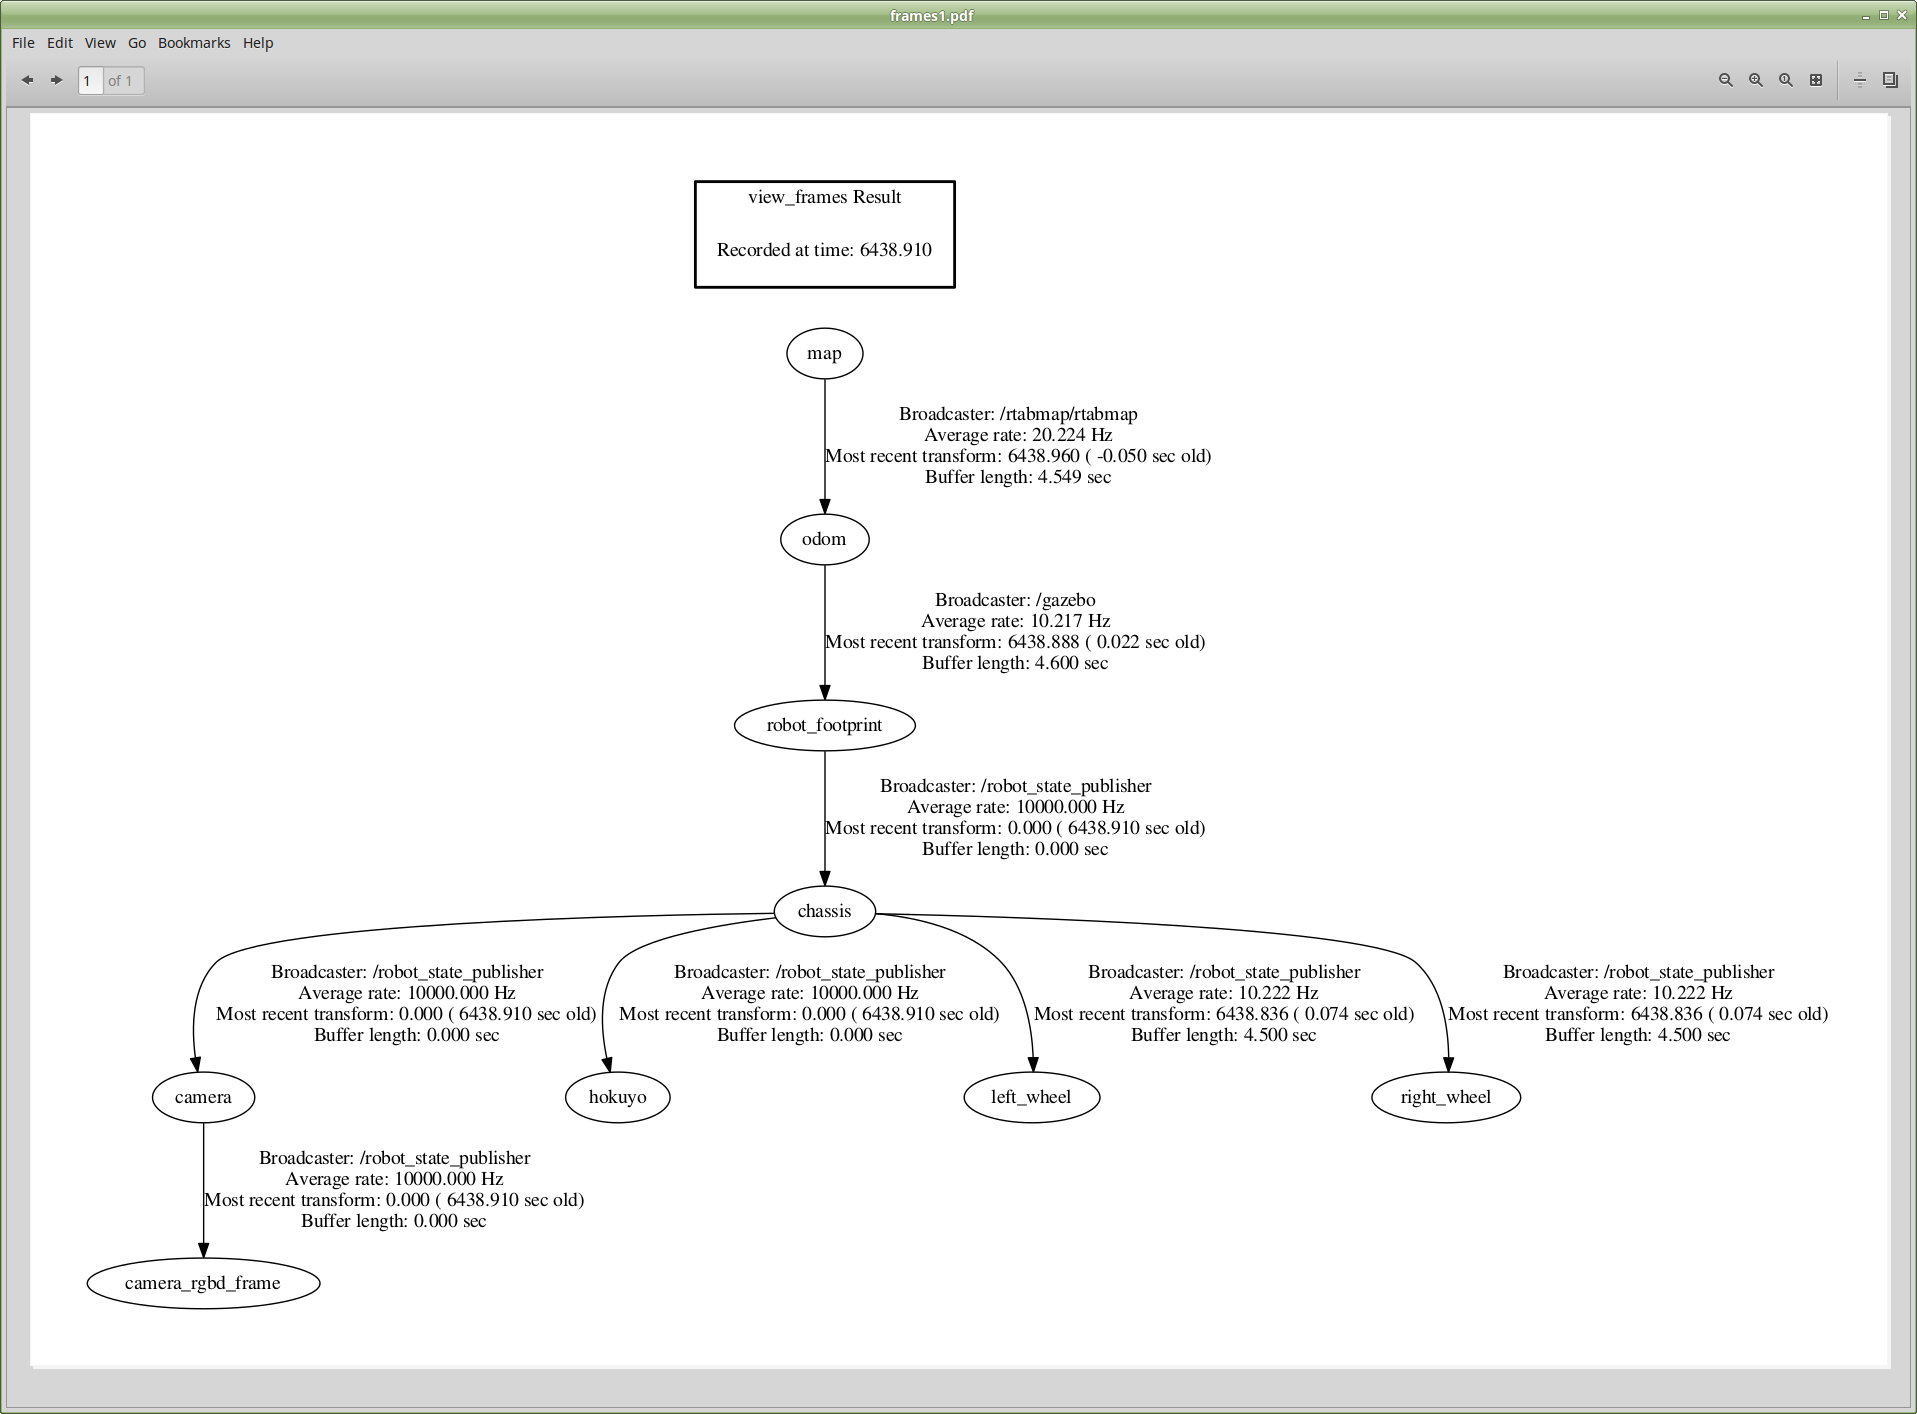
\includegraphics[width=\linewidth]{Assets/Frames1_ScreenShot_2019-02-12_16-25-23.png}
      \caption{CielBot Transform Tree}
      \label{fig:tftree}
\end{figure}


\subsection{Custom World Config}
The custom world was created with Gazebo. Using Gazebo for world editing was unintuitive and for this reason a very simple world was designed. It is a L shaped building of variously colored walls with a variety of predefined object models placed at random around the room as seen in Fig ~\ref{fig:customworld}.

\begin{figure}[h]
      \centering
      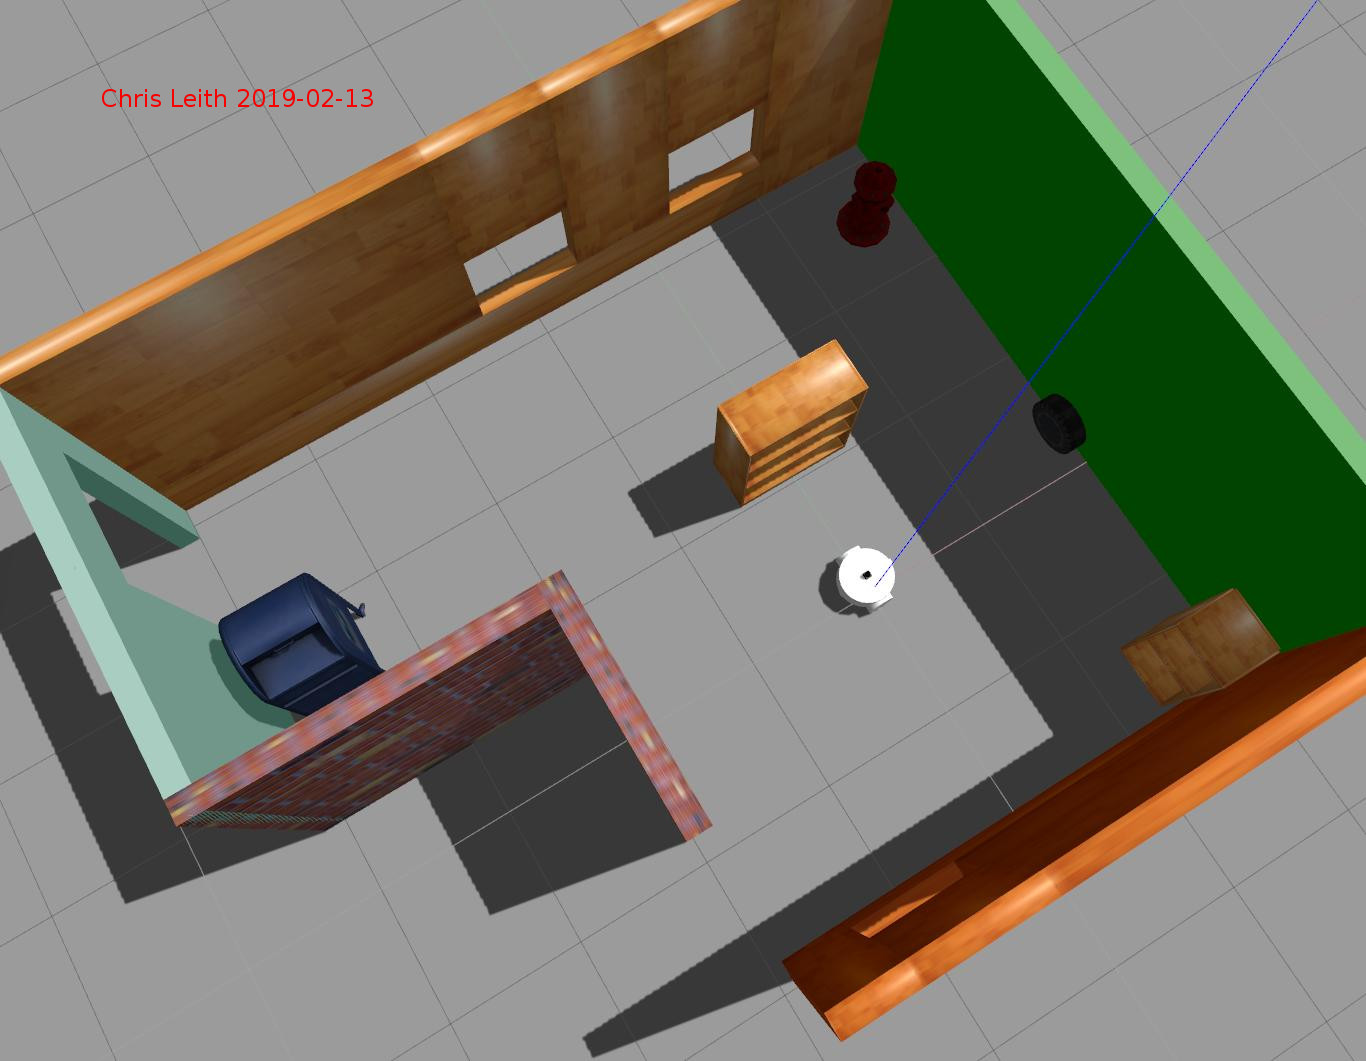
\includegraphics[width=\linewidth]{Assets/custom_gazebo_world.jpg}
      \caption{Custom World}
      \label{fig:customworld}
\end{figure}

\section{Results}
Map generation was reasonable, but not perfect as detailed below.
\subsection{Results - Kitchen and Dining World}
From Run1 Fig ~\ref{fig:kitchen_dbview_run1} it is seen that RTABMap was able to detect 78 loop closures and generated a reasonably clean occupancy grid, but with some obvious flaws. The 2D map shows that most loop closures were concentrate in one part of the kitchen with none in the dining room. This is most likely due to the fact that the kitchen was traversed 3 times and the dining room only once.


\begin{figure}[h]
      \centering
      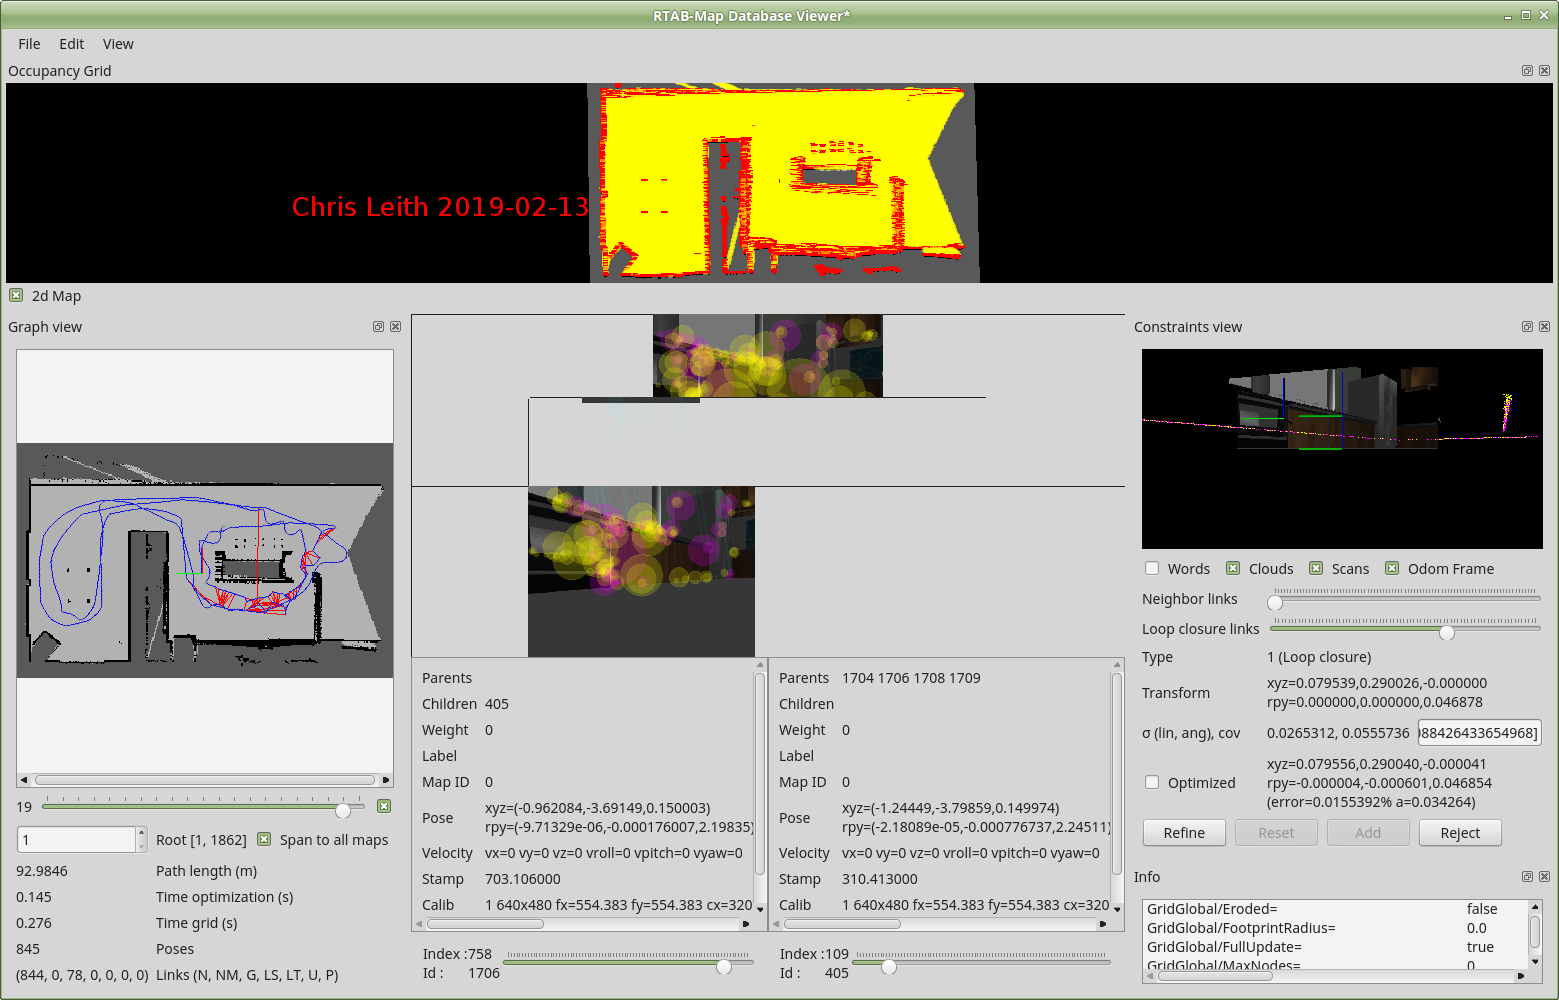
\includegraphics[width=\linewidth]{Assets/DBViewer_kitchen_2019-02-11_19-04-25.png}
      \caption{Kitchen and Dining World DBView Run1}
      \label{fig:kitchen_dbview_run1}
\end{figure}

From Run2 Fig ~\ref{fig:kitchen_dbview_run2} it is seen that RTABMap was able to detect 46 loop closures and generate a recognizable 3D map. However, again some flaws are evident. For example it is evident that RTABMap was unable to detect the correspondence of the stool images and there are thus 'ghost' stool images.

\begin{figure}[h]
      \centering
      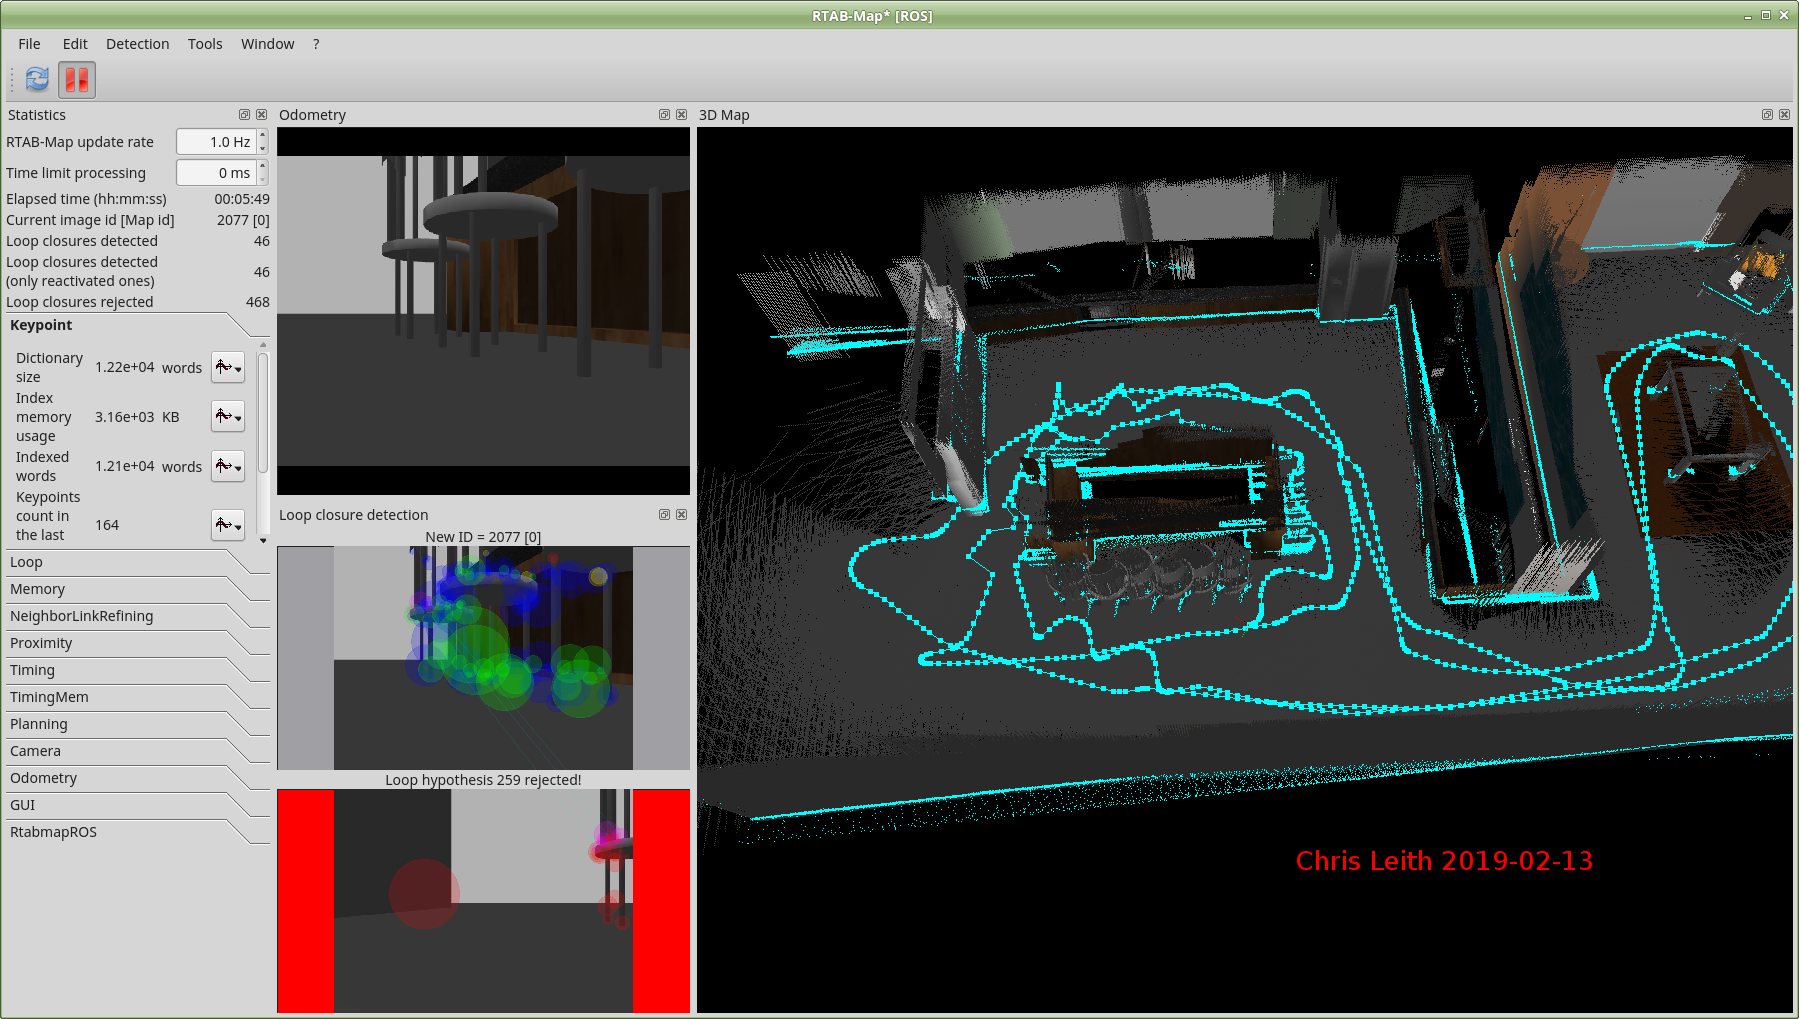
\includegraphics[width=\linewidth]{Assets/rtabviz_kitchen46LC_2019-02-11_19-04-25.png}
      \caption{Kitchen and Dining World DBView Run2}
      \label{fig:kitchen_dbview_run2}
\end{figure}

\subsection{Results - Custom World}
From Fig ~\ref{fig:customworld_Map_3D} it can be seen that RTABMap was able to establish 67 loop closures and to generate a recognizable 3D map (compare to Fig ~\ref{fig:customworld}) it is clear from Fig ~\ref{fig:customworld_Map_2D} that the map creation was not robust.



\begin{figure}[h]
      \centering
      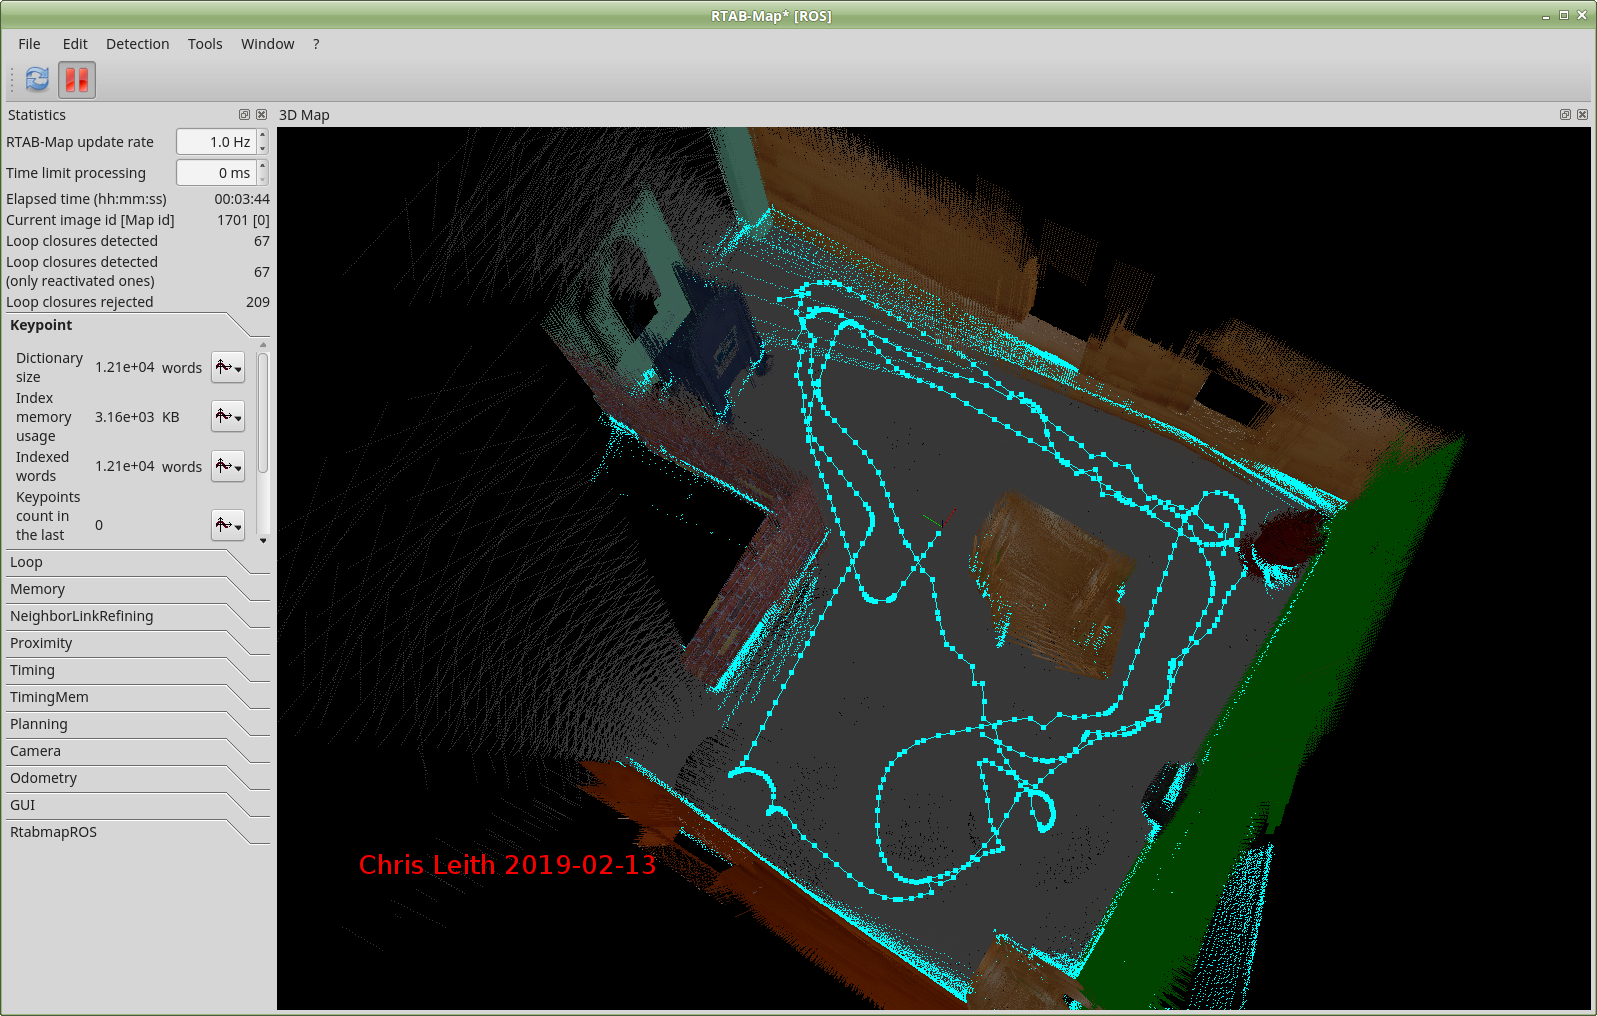
\includegraphics[width=\linewidth]{Assets/RTabViewMap_Custom.png}
      \caption{Custom World 3D Map}
      \label{fig:customworld_Map_3D}
\end{figure}

\begin{figure}[h]
      \centering
      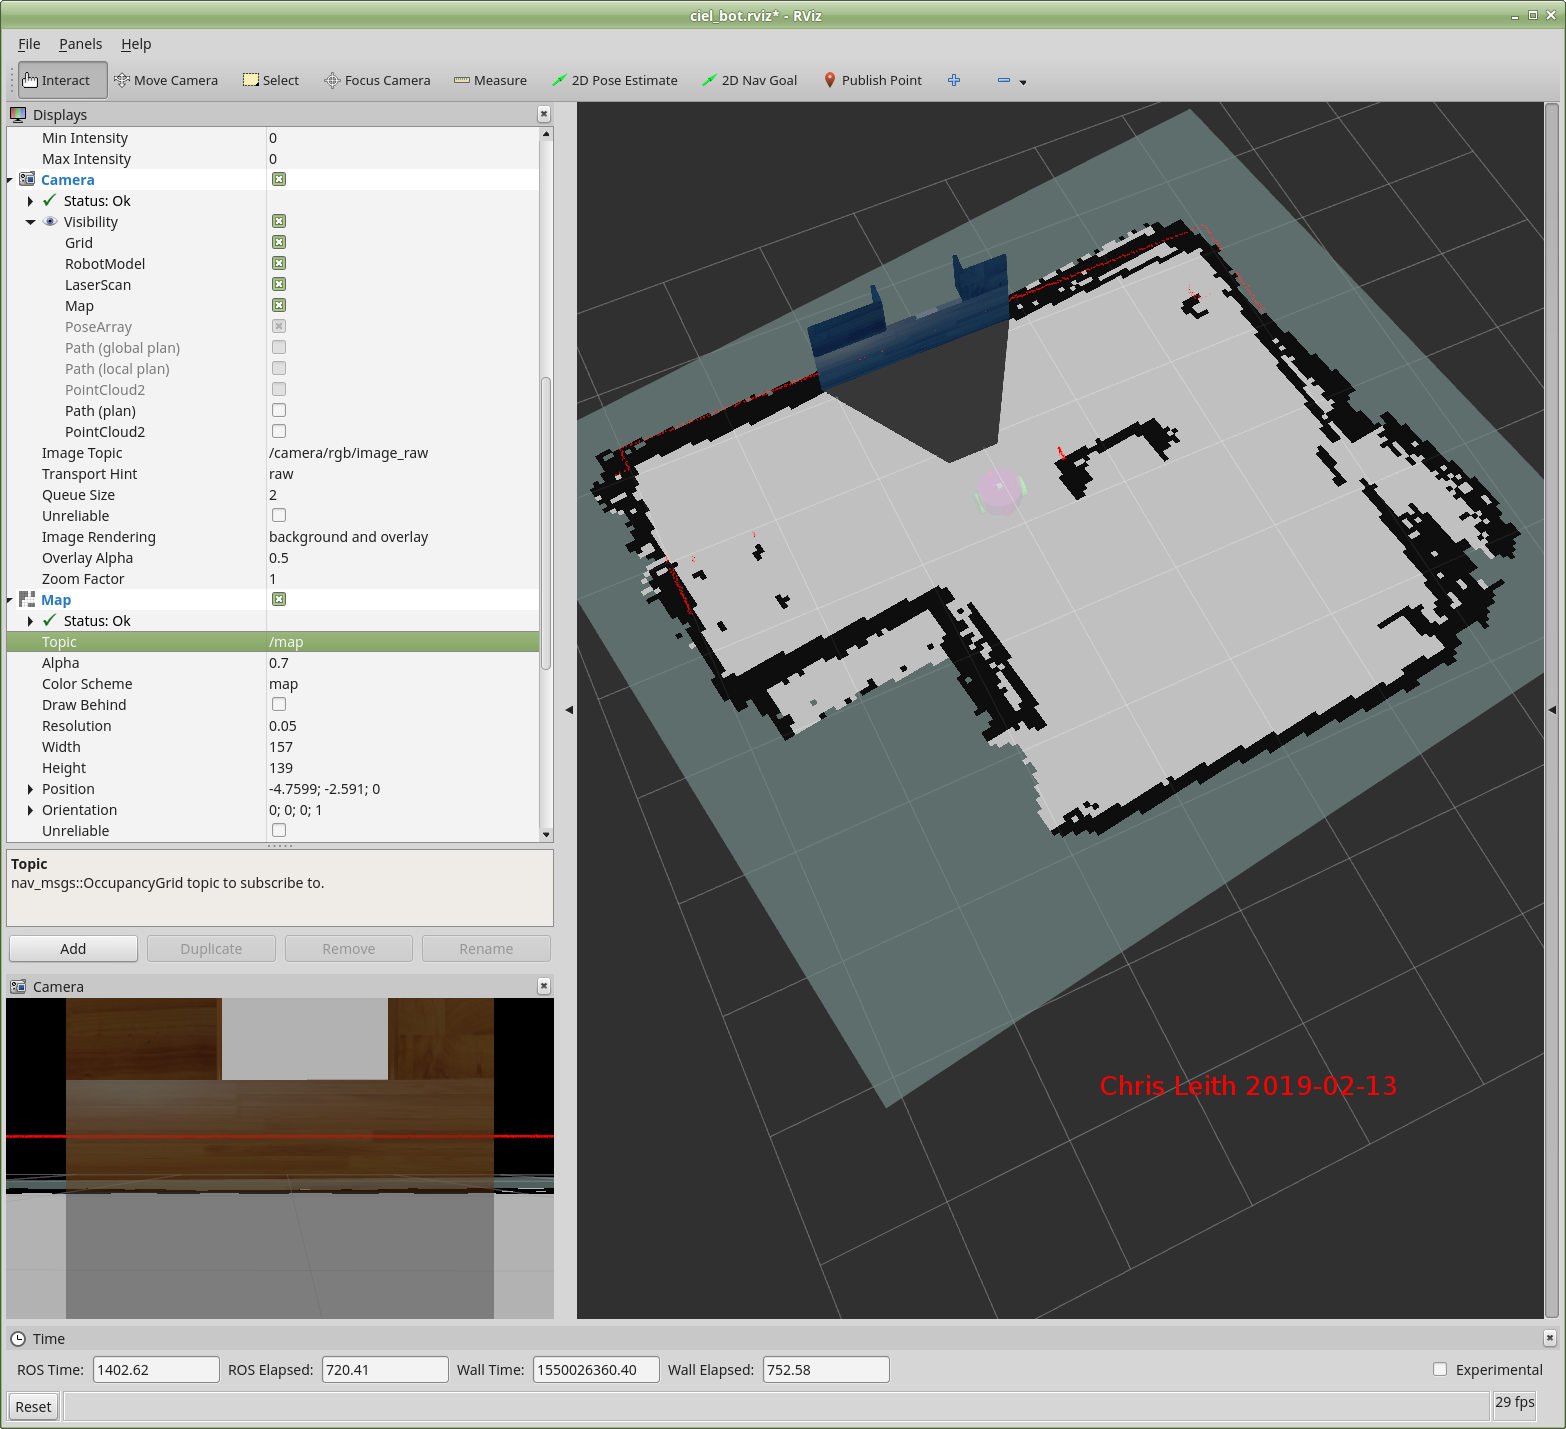
\includegraphics[width=\linewidth]{Assets/rviz_custom_map.png}
      \caption{Custom World 2D Map}
      \label{fig:customworld_Map_2D}
\end{figure}



\section{Discussion}
The maps generated in all cases had flaws. However these were an improvement over prior runs where the robot made fewer traversals. It is almost certain that yet more traversals would generate improved results. However, there was a time shortage that prevented further efforts on improving the mapping results. For example, as mentioned in the Config Section, there are numerous RTABMap parameters that could be optimized.

In some earlier expermental simple worlds it was observed that simple, uniform or symmetric worlds present more difficulty to SLAM than richer, more complex environments. By adding more objects to the custom world, and more features such as color and texture, mapping results could be improved. However there is likely a 'sweet spot' of feature richness beyond which the complexity af comparing features, especially in a large environment, would become computational very difficult and require heavy computational resources.

\section{Conclusion / Future work}
The project was modestly successful in terms of simple simple goal of implementing a robot that uses RTABMap in ROS/Gazebo to perform SLAM mapping and localization in a simple simulated enviroenment. It was also modestly successful in terms of the wider goal of gaining experience and increased understanding of SLAM and it's subleties and the ROS/Gazebo environment as a robot design and test platform. Unfortunately the mechanincs of getting ROS and various dependencies configured and the difficulty in finding help for simple errors meant that no time was left for actually exploring the behaviour of the SLAM solution or exploring further reading about various SLAM techniques. Those would be useful pursuits in the future.

In particular parameters tuning could optimize for accurate, precise localization and mapping, or for improved processing time to permit running on less powerful robots. 

Future work could include integrating other sensors into the robot, eg IMUs, radar, ultrasonic rangers, GPS and more. Also using a more challenging map and more challenging goals like waypoint navigation around the entire map. And of course the real challenge will be to implement the whole design on a real robot running ROS in the real world. It would be great fun but surely many unexpected challenges would arise including many discreapancies between running ROS in the real world versus running ROS in the Gazebo environment. 

\end{document}